\chapter{Optimizing the CNN}%\label{make}

\section{Processing the Images}
For the following steps, a simulated dataset containing roughly \num{800000} gamma events
and \num{400000} hadron events has been used.
Each recorded event holds the counts of every arrived photon for all \num{1440} pixels
for \num{100} consecutive time frames of \num{0.5}\,\si{\nano\second}.
To reduce these \num{144000} variables,
the counts of photons for each pixel have been summed along the time axis (time series summation).

\begin{figure}
    \centering
    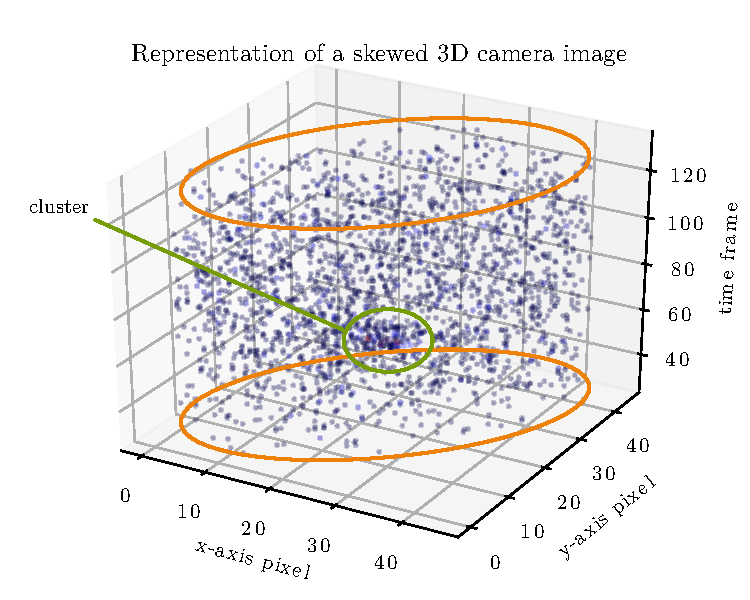
\includegraphics[scale=0.75]{Plots/3d_Camera_Image.pdf}
    \caption{An event contains \num{100} consecutive images of the Cherenkov flash. To minimize the number of variables, all values for a single pixel have been summed up for each event.}
    \label{fig:example_event}
\end{figure}

Naturally, many background photons are contained in the image.
Since the telescope triggers all events in approximately the same time frame,
the photons of the air shower can be cut out by removing preceding and succeeding time frames filled with noise.
This results in cleaner, denoised images for the pattern detection in the CNN.

\begin{figure}
    \centering
    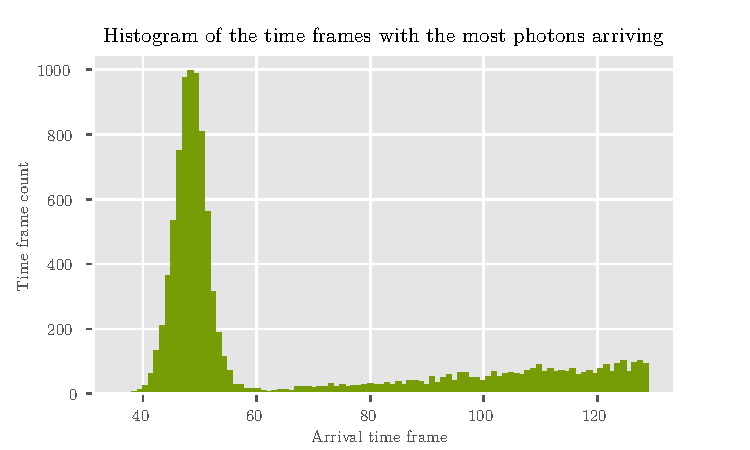
\includegraphics[scale=1]{Plots/Arrivaltimes.pdf}
    \caption{The brightest time frames for \num{10000} events are shown in the histogram. The distribution peaks around the triggering time. By cutting out this cluster, noise can be reduced.}
    \label{fig:arrivaltimes}
\end{figure}

For \num{10000} events, the time frame with the most photons arriving was computed.
These bright time frames most likely contain the events to examine.
Creating a histogram of these time frames,
highlights that the telescope triggers the events between frames \num{35} and \num{60} nearly every time.
As a result, only this range of frames will be used for the denoised images,
dropping all other frames, which contain mostly noise.

In the following paragraph, all architectures will be evaluated on the images
containing all photons as well as the denoised ones.


\section{Comparing Architectures}
In this section each tested network architecture is composed of a convolution layer followed by a pooling layer (c)
and fully-connected layers (f).
The architecture notation follows this example:

\begin{itemize}
\item A \enquote{\texttt{3c\_2f}} architecture translates to a network
starting with three convolution-and-pooling layers and ending with two fully connected layers.
\end{itemize}

There are four important hyperparameters for networks of this kind:

\begin{itemize}
\item The number of images in one batch fed to the network (batch-size)
\item The size of the patch/kernel in the convolution layers (patch-size)
\item The number of feature maps the convolution layers compute (depth)
\item The number of neurons contained in the fully-connected layers (neurons)
\end{itemize}

For all parameters a random grid search was performed over the course of the following steps.
To reduce the impact of random fluctuations in the network's performance caused inter alia by the grid search,
\num{50} networks have been trained for each architecture.

The common procedure of using a separate training, validation and testing dataset has been adopted.
To measure the network's performance, the area under the Receiver-Operating Characteristic (ROC-AUC) \cite{roc_auc} is used.
The training of a network is terminated when the ROC-AUC-score of the validation dataset does not rise anymore (early stopping).

\begin{figure}
\centering
\begin{subfigure}{.5\textwidth}
  \centering
  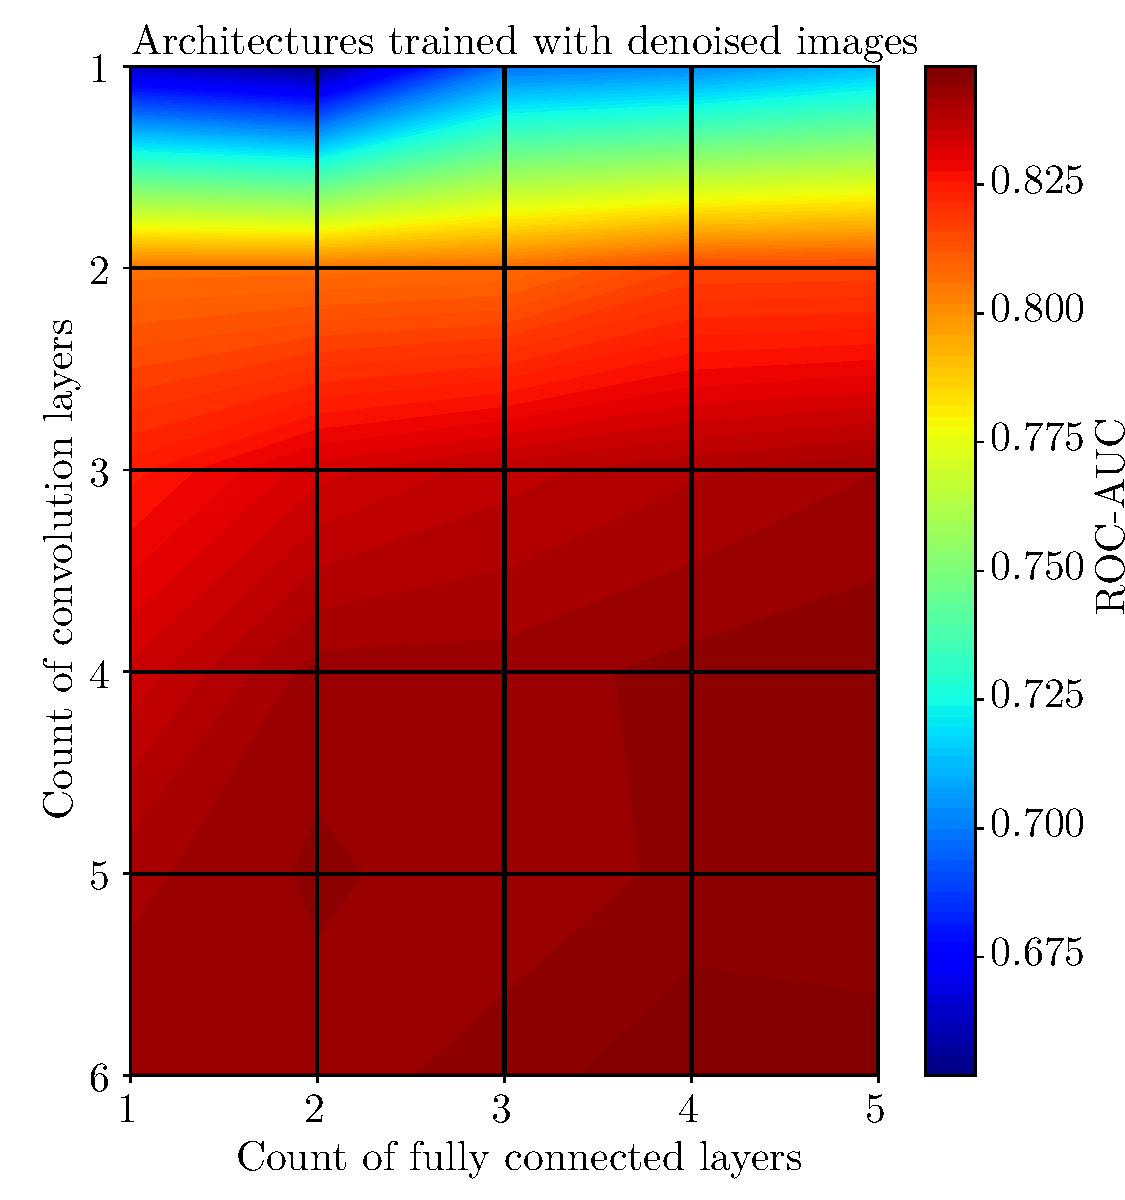
\includegraphics[scale=0.35]{Plots/Architectures_AUC_denoised.pdf}
  \caption{CNNs on denoised images}
  \label{fig:heatmap_denoised}
\end{subfigure}%
\begin{subfigure}{.5\textwidth}
  \centering
  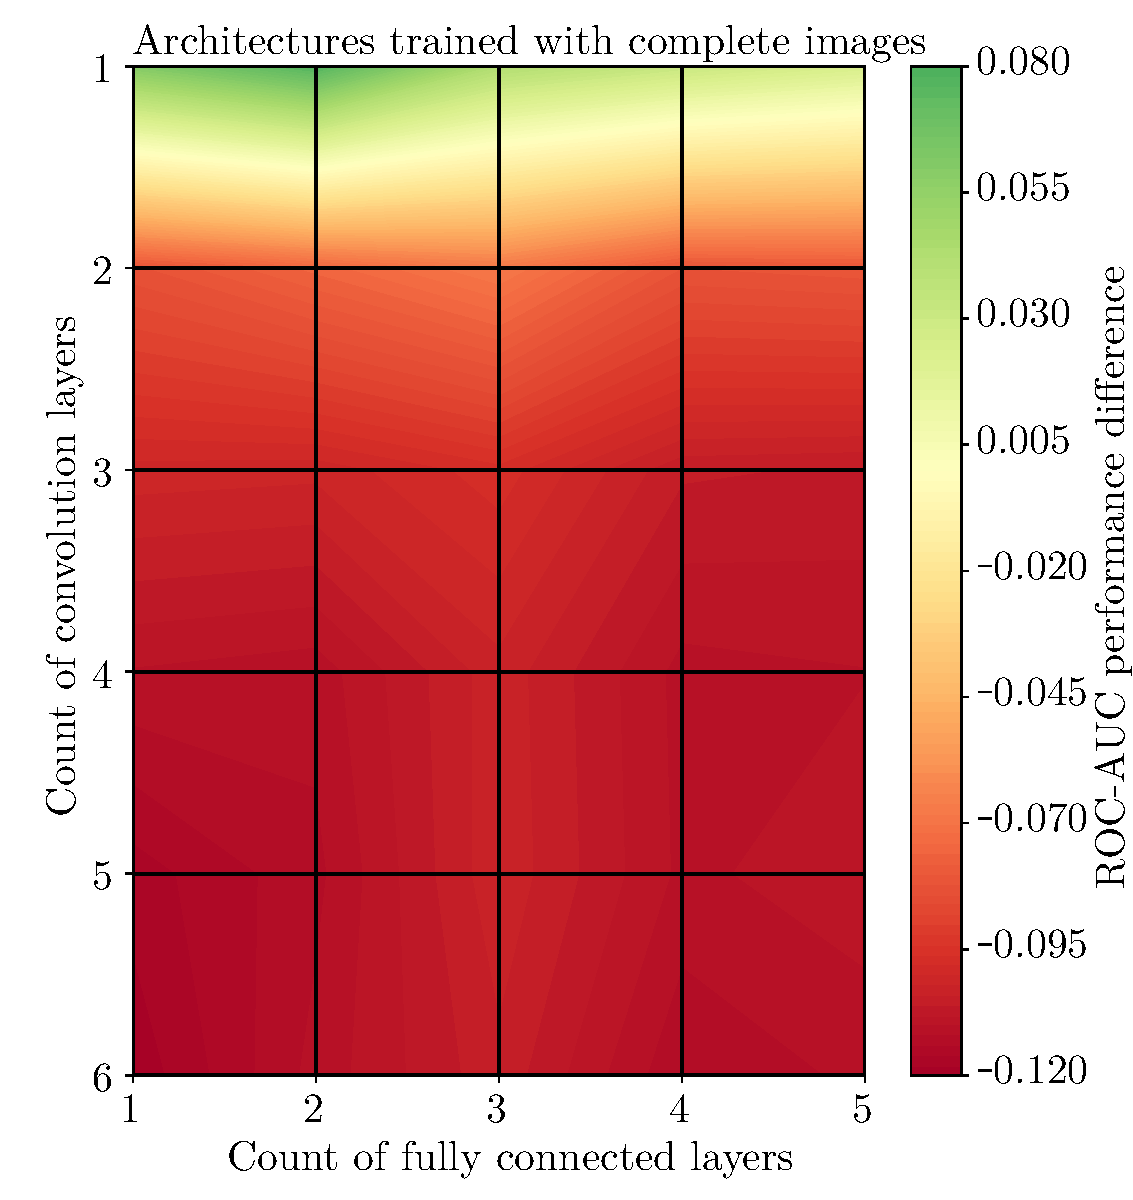
\includegraphics[scale=0.35]{Plots/Architectures_AUC_noised.pdf}
  \caption{CNNs on noisy images}
  \label{fig:heatmap_noised}
\end{subfigure}
\caption{The ROC-AUC performances of \num{30} architectures are compared on both denoised and noisy images. Since denoised images perform better, the second plot shows the difference between the denoised and noisy images' ROC-AUC scores.}
\label{fig:heatmaps}
\end{figure}

By comparing the networks trained on noisy and denoised images, it becomes apparent
that denoised images produce a much more reliable and therefore better network.

Looking at the architectures, it appears unambiguous that deeper networks perform much better than shallow ones.
The number of feature-generating convolution layers seems to have a greater impact
than the number of fully connected layers on the ROC-AUC score.

By examining the best-performing denoised deep network architectures,
only sleight differences can be seen.
Since a sample of only \num{50} trained networks guarantees no statistical certainty,
no distinct best architecture can be proclaimed.

\begin{figure}
    \centering
    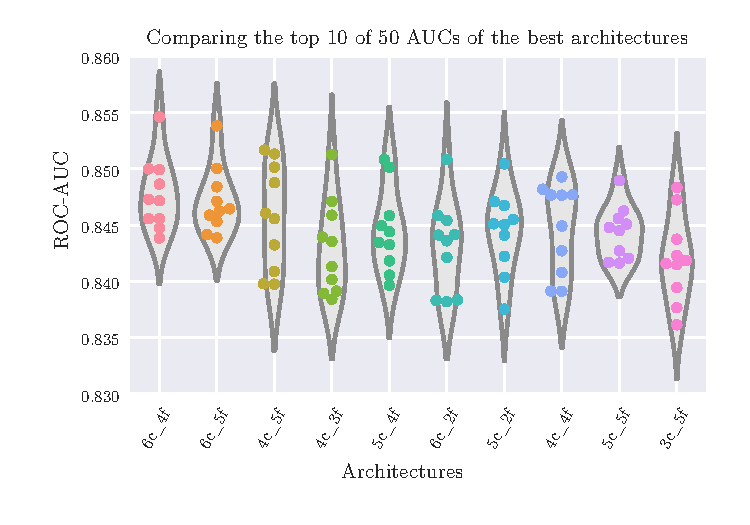
\includegraphics[scale=1]{Plots/Best_denoised_architectures.pdf}
    \caption{For the comparison of the best denoised architectures the \num{10} best performing networks from \num{50} are being compared in this plot.}
    \label{fig:top_cnn_architectures}
\end{figure}

It can be seen that deeper networks perform better on the given task
and the more convolution layers included in the architecture, the higher the ROC-AUC score.
Additionally, using only the important part of the recorded events
and dropping some noise, increases the network's performance as well.

For a meaningful conclusion concerning the architectures, the hyperparameters of the networks will be investigated.
Since the optimal values for the hyperparameters could not be determined beforehand,
all parameters for the above investigations were randomly chosen from a suitable value range.
Therefore a conclusion can be drawn afterwards to narrow this range down or investigate a more promising value range.

Since only the best networks are of interest, the hyperparameters of the high performing ones are investigated.
For this analysis, the performance of all computed networks are compared regardless of their architecture.
As all parameters (batch-size, patch-size, depth and neurons) show only a small impact on the ROC-AUC score,
only small gains in performance can be achieved through optimizing the hyperparameters.
For this reason the random grid search will be performed for further investigations.

\begin{figure}
\centering
\begin{subfigure}{.5\textwidth}
  \centering
  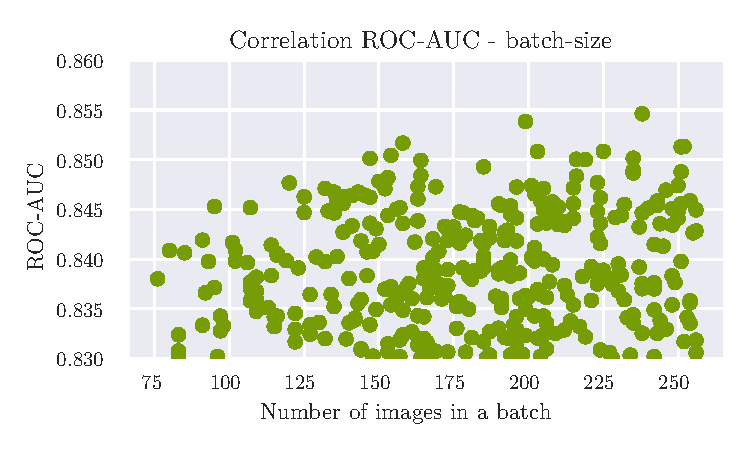
\includegraphics[scale=0.55]{Plots/Best_Hyperparameter_Batch_Size.pdf}
  \caption{Parameter batch-size}
  \label{fig:batch_size}
\end{subfigure}%
\begin{subfigure}{.5\textwidth}
  \centering
  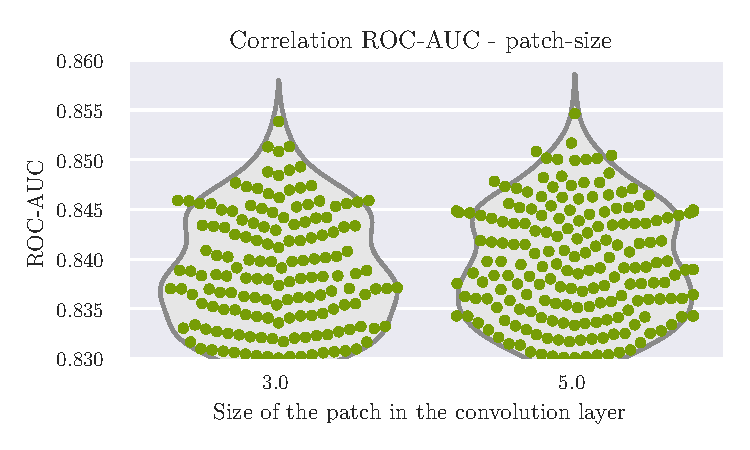
\includegraphics[scale=0.55]{Plots/Best_Hyperparameter_Patch_Size.pdf}
  \caption{Parameter patch-size}
  \label{fig:patch_size}
\end{subfigure}

\centering
\begin{subfigure}{.5\textwidth}
  \centering
  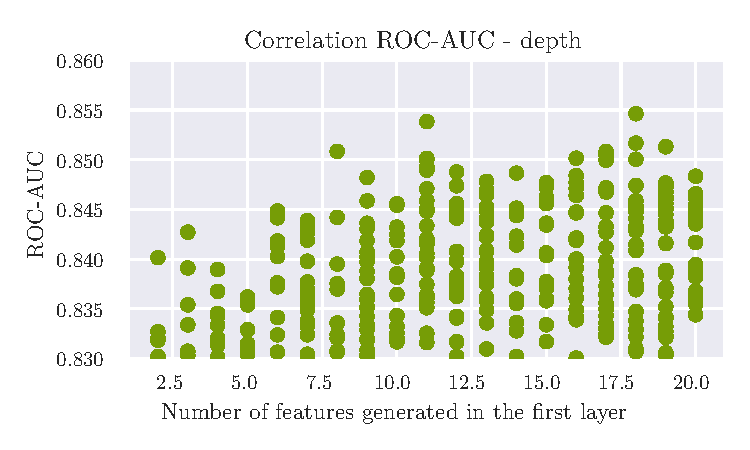
\includegraphics[scale=0.55]{Plots/Best_Hyperparameter_Depth_1.pdf}
  \caption{Parameter depth (first c-layer)}
  \label{fig:depth}
\end{subfigure}%
\begin{subfigure}{.5\textwidth}
  \centering
  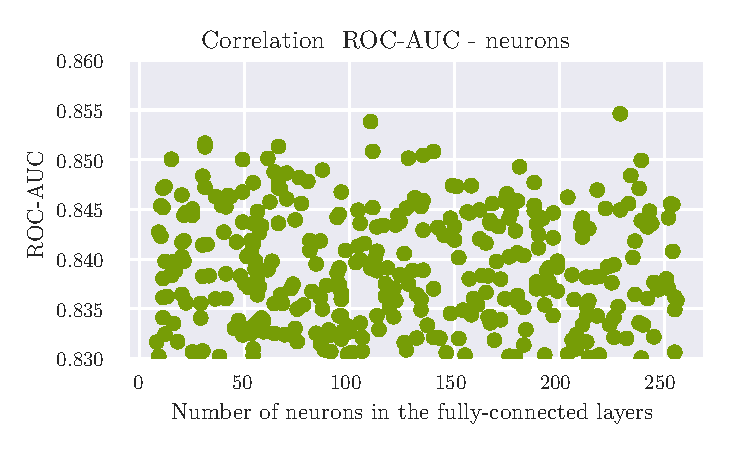
\includegraphics[scale=0.55]{Plots/Best_Hyperparameter_Hidden_Nodes.pdf}
  \caption{Parameter hidden-nodes}
  \label{fig:hidden_nodes}
\end{subfigure}
\caption{Only a small impact on the ROC-AUC can be detected by comparing the hyperparameters. Since optimizing the parameters specifically appears complicated, the random grid search will be utilized henceforth.}
\label{fig:parameter}
\end{figure}



\section{Regularizing the Network}
The best-performing \enquote{\texttt{6c\_4f}} architecture is fixed for further investigations
so that the feature space to explore is reduced.
To stabilize behavior of the network, regularizing dropout layers will be integrated into the network's architecture.

Since the layer can be combined with every existing layer in the network
and can likewise adopt different values for the amount of data to drop out in every layer,
a large feature space has to be evaluated.
As adding dropout to a network extends the training time many times over,
only one dropout layer at once can be tested at every position.
In the first round of testing, a dropout rate of \num{50}\,\% will be used.
Investigating every possible permutation of multiple dropout layers is not possible
because of the size of the feature space that must be explored.

\begin{figure}
    \centering
    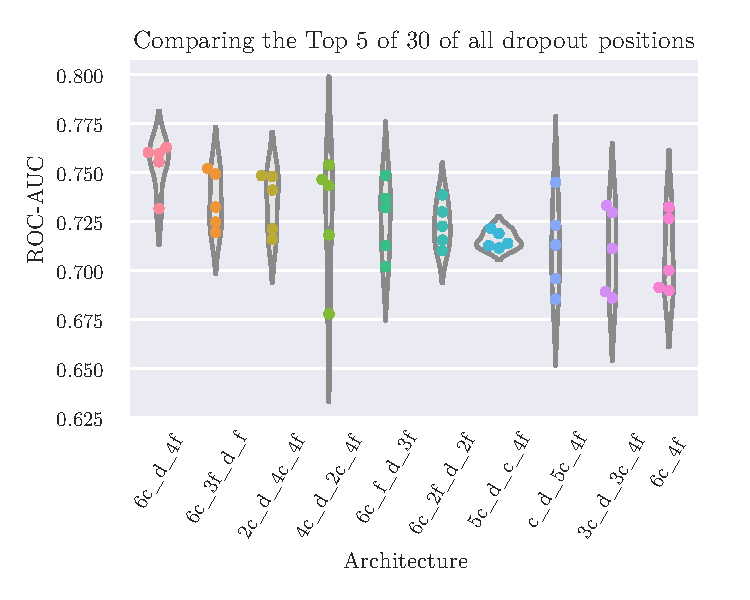
\includegraphics[scale=1]{Plots/Dropout_Positions.pdf}
    \caption{Using dropout layers increases the performance every time, but inserting the layer between the convolution and the fully connected layers, unlocks its potential the most.}
    \label{fig:random_dropout}
\end{figure}

Positioning the dropout layer between the convolution layers and the following fully-connected layers
appears to have the most positive impact on the network's performance.
Regularizing the fully connected layers seems to strengthen the network as well.
On the contrary, dropping too much information in the convolution layers weakens the network overall.
Therefore, the dropout rate is most important, when it is combined with the layer's position.

It has been decided that dropout layers shall be implemented after every layer, but using different dropout rates.
The rates in table \ref{tab:dropout_rates} were taken from corresponding literature \cite{deeplearning}.

\begin{table}
    \centering
    \caption{The chosen dropout rates for the different dropout positions}
    \label{tab:dropout_rates}
    \begin{tabular}{cc}
        \toprule
        {Dropout position}  & {Dropout rate} \\
        \midrule
        c- d -c & 0.90 \\
        c- d -f & 0.75 \\
        f- d -f & 0.50 \\
        \bottomrule
    \end{tabular}
\end{table}

Since dropout prolongs the network's training cycle and increases the difficulty of training deep networks in general,
pretraining is used to enable efficient training of many layers.

A short network containing dropout layers is trained for a few epochs
and the layers adjust their inner values using gradient decent.
Afterwards new layers are appended to the network and the short training epoch starts again.
In this case training epochs consisting of \num{0}, \num{1000}, \num{2000}, \num{5000} and \num{8000} batches are being compared.
To complete the training after the network has grown to its full depth, a normal training epoch with early stopping is used.

\begin{figure}
    \centering
    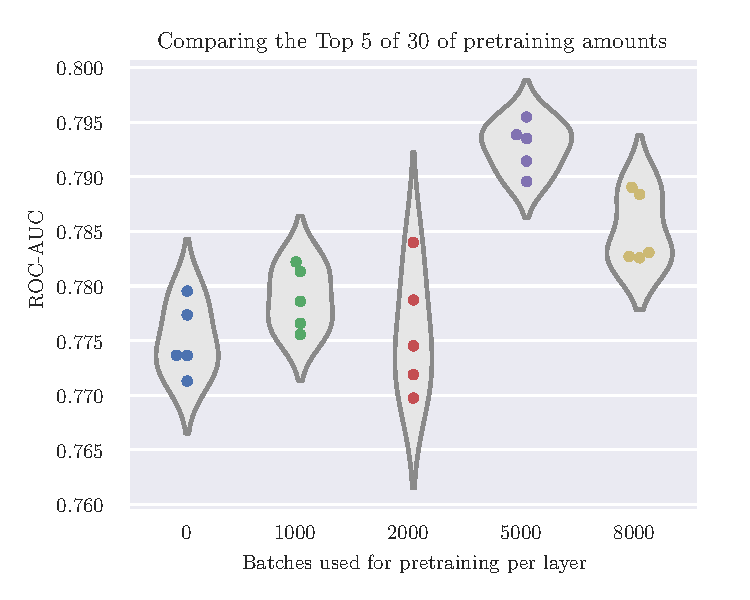
\includegraphics[scale=1]{Plots/Pretraining_Amounts.pdf}
    \caption{Implementing pretraining in the training process increases the network's performance in general. Since too much pretraining appears to be counterproductive, \num{5000}\,batches will be used henceforth.}
    \label{fig:pretraining_amounts}
\end{figure}

Using different amounts of pretraining batches, the results illustrate an increase in the performance
when compared to the networks without pretrained layers.
By pretraining the network too much, there seems to be an decrease in the performance through overfitting.
Therefore, it is advisable to choose the pretraining amount carefully.
In this case \num{5000} batches of images have been chosen.
